\documentclass[article, bachelor, och, pract]{SCWorks}


\usepackage[utf8]{inputenc}
%\usepackage[T2A]{fontenc}
\usepackage{amsthm,amsmath,amssymb,amsfonts}
\usepackage[russian]{babel}
\usepackage{indentfirst}
%%%%%%%%%%%%%%%%%%%%%
\usepackage{graphicx}
\graphicspath{{pictures/}}
\DeclareGraphicsExtensions{.png,.jpg}


%\usepackage[colorlinks=true]{hyperref}

\begin{document}

\chair{дифференциальных уравнений и прикладной математики}
\worktitle{}
\course{2}

\group{213}




\chtitle{д.ф-м.н., доцент} 
\chname{}  
%\patitle{} 
%\paname{}
%\term{} 



\napravlenie{01.03.02 "Прикладная математика и информатика"}

\studentName{Шарова Александра Вадимовича}

\practStart{1 Июля 2016}  
\practFinish{14 Июля 2016} 

\satitle{к.ф.-м.н., доцент}
\saname{В. А. Халова}

\year{2016}  
\MakeTitle

\setcounter{tocdepth}{1}

\tableofcontents
\intro


Цель данной практики - изучить основы работы в системе компьютерной математике Maxima. 


\section{Простые вычисления}
Упростить выражения: № 1.013, № 1.028, № 1.043 [Из сборника задач по математике для поступающих во втузы, под редакцией Сканави М. И.]. Для упрощения выражения воспользуемся командой \textbf{ratsimp(Функция)}.
\\

№ 1.013\\
Упростить выражение:

$(x^2+2x-\frac{11x-2}{3x+1}):(x+1-\frac{2x^2+x+2}{3x+1}); \; \; x=7,(3)$

\texttt{ratsimp((x\^{}2+2*x+(11*x-2)/(3*x+1))/(x+1-(2*x\^{}2+x+2)/(3*x+1)));}\\
%%%%%%%%%%%%%%%
Ответ: $\frac{-2+13x+7x^2+3x^3}{x^2+3x-1}$
%%%%%%%%%%%%%%%
\\
Вычислим при $x = 3:$

\texttt{ratsubst(3, x, (-2+13*x+7*x\^{}2+3*x\^{}3)/(x\^{}2+3*x-1));}\\
%%%%%%%%%%%%%%%
Ответ: $\frac{181}{17}$
%%%%%%%%%%%%%%%
\\
Вычислим при $x = 7:$

\texttt{ratsubst(7, x, (-2+13*x+7*x\^{}2+3*x\^{}3)/(x\^{}2+3*x-1));}\\
%%%%%%%%%%%%%%%
Ответ: $\frac{487}{23}$
%%%%%%%%%%%%%%%
\\

№ 1.028\\
Упростить выражение:

$ \frac{\left(\sqrt[3]{\sqrt{(r^2+4)\sqrt{1+\frac{4}{r^2}}}}-\sqrt[3]{\sqrt{(r^2-4)\sqrt{1-\frac{4}{r^2}}}}\right)^2}{r^2-\sqrt{r^4-16}}$


\texttt{ratsimp((((r\^{}2+4)*sqrt(1+4/r\^{}2))\^{}(1/3)\\-((r\^{}2-4)*sqrt(1-4/r\^{}2))\^{}(1/3))/(r\^{}2-sqrt(r\^{}4-16)));}\\

Ответ:
$-\frac{\sqrt{r^2+4}-\sqrt{r^2-4}}{\sqrt{r^4-16}|r|^{\frac{1}{3}}-r^2|r|^{\frac{1}{3}}}$
%%%%%%%%%%%%%%%
\\

№ 1.043\\
Упростить выражение:
$$ \frac{x-1}{x+x^{0.5}+1}:\frac{x^{0.5}+1}{x^{1.5}-1}+\frac{2}{x^{-0.5}}$$
\texttt{ratsimp(((x-1)/(x+x\^{}(1/2)+1))/((x\^{}(1/2)+1)/(x\^{}(3/2)-1))+2/(x\^{}(-1/2)));}\\
Ответ: 
$x+1$

%%%%%%%%%%%%%%%

\newpage
\section{Алгебра матриц}
\begin{itemize}
\item[1.] Найти произведение матриц A и B. Произведение двух матриц в \emph{Maxima} обозначается символом "."\\
$$
A=\begin{pmatrix}
1 & 2 & 2 & -1\\
2 & 3 & 4 & 5\\
1 & 3 & 2 & 5\\
3 & 2 & 4 & -3
\end{pmatrix}; \; \; \;
B=\begin{pmatrix}
-5 & 2 & -1\\
-1 & 7 & 3\\
-2 & 4 & -3\\
1 & 3 & 2
\end{pmatrix}$$\\
\texttt{A: matrix([1,2,2,-1],[2,3,4,5],[1,3,2,5],[3,2,4,-3]);}\\
\texttt{B: matrix([-5,2,-1],[-1,7,3],[-2,4,-3],[1,3,2]);}
%%%%%%%%%%%%%%%
\\
$$A.B = 
\begin{pmatrix}
-12 & 21 & -3\\
-16 & 56 & 5\\
-7 & 46 & 12\\
-27 & 27 & -15 \\
\end{pmatrix}$$
%%%%%%%%%%%%%%%
\item[2.] Вычислить определитель матрицы A. Для подсчета определителя матрицы воспользуемся командой \textbf{determinant(A)}.\\
$$\begin{pmatrix}
1 & 2 & 3 & 4 & 5\\
2 & 3 & 7 & 10 & 13\\
3 & 5 & 11 & 16 & 21\\
2 & -7 & 7 & 7 & 2\\
1 & 4 & 5 & 3 & 10 \\
\end{pmatrix}$$\\
\texttt{determinant(matrix([1,2,3,4,5],[2,3,7,10,13],[3,5,11,16,21],}\\
\texttt{[2,-7,7,7,2],[1,4,5,3,10]));}\\
%%%%%%%%%%%%%%%
Ответ: 52



\item[3.] Дана матрица A. Найти матрицу \(A^{-1}\) и установить, что \(AA^{-1}=E\). Для начала обратим матрицу А, и запишем ее как матрица B. Чтобы обратить матрицу, существует команда \textbf{invert(A)}.\\
\texttt{A: matrix([17,10,4],[1,1,0],[2,-3,3]);}\\
$$A=\begin{pmatrix}
17 & 10 & 4 \\
1 & 1 & 0 \\
2 & -3 & 3 \\
\end{pmatrix}
$$\\

\texttt{B: invert(A);}\\
%%%%%%%%%%%%%%%
$$B=\begin{pmatrix}
3 & -42 & -4 \\
-3 & 43 & 4 \\
-5 & 71 & 7 \\
\end{pmatrix}$$\\
%%%%%%%%%%%%%%%
Покажем, что произведение матриц A и B есть единичная матрица:\\
$$A.B=\begin{pmatrix}
1 & 0 & 0\\
0 & 1 & 0\\
0 & 0 & 1
\end{pmatrix}$$\\
Получили единичную матрицу.
%%%%%%%%%%%%%%%
\end{itemize}

\newpage
\section{Функции математического анализа}
\begin{itemize}
\item[1.] Найти пределы выражений: № 746, № 761, № 776 [Из сборника задач по высшей математике, Минорский В. П.]. Для нахождения предела воспользуемся командой \textbf{limit(функция, переменная, точка)}.

№ 746\\
Найти предел:
$$\lim_{x \to \infty}\frac{2x^2-1}{3x^2-4x}$$
Запишем функцию:
$$F=\frac{2x^2-1}{3x^2-4x}$$

\texttt{F: (2*x\^{}2-1)/(3*x\^{}2-4*x);}\\
\texttt{limit(F, x, $\infty$)}; \\ 
Ответ: $\frac{2}{3}$

№ 761\\
Найти предел:
$$\lim_{x \to 7}\frac{2-\sqrt{x-3}}{x^2-49}$$
Запишем функцию:
$$F=\frac{2-\sqrt{x-3}}{x^2-49}$$

\texttt{F: (2-sqrt(x-3))/(x\^{}2-49);}\\
\texttt{limit(F, x, 7)}; \\ 
Ответ: $-\frac{1}{56}$

№ 776\\
Найти предел:
$$\lim_{x \to 0}\frac{2x\sin{x}}{\sec{x}-1}$$
Запишем функцию:
$$F=\frac{2x\sin{x}}{\sec{x}-1}$$

\texttt{F: (2*x*sin(x))/(sec(x)-1);}\\
\texttt{limit(F, x, 0)}; \\ 
Ответ: $4$

\item[2.] Вычислить производные: № 886, № 901 [Из сборника задач по высшей математике, Минорский В. П.]. Для вычисления производной воспользуемся командой \textbf{diff(y(x), x)}, где y(x) - функция, x - переменная, по которой дифференцируем.

№ 886\\
Найти производную функции:\\
1) Дана функция: $$ y = \frac{1}{(1+\cos{4x})^5} $$
\texttt{y(x):=1/(1+cos(4*x))\^{}5;}\\
\texttt{diff(y(x),x);}\\
Ответ: \[\frac{20\sin{(4x)}}{{{\left( 1+\cos{(4x)}\right) }^{6}}}\]

%%%%%%%%%%%%%%%

2) Дана функция: $$ s = \sqrt{\frac{t}{2} - sin{\frac{t}{2}}} $$
\texttt{s(t):=sqrt(t/2-sin(t/2))}\\
\texttt{diff(s(t),t);}\\
Ответ:
\[\frac{\frac{1}{2}-\frac{\cos{\left( \frac{t}{2}\right) }}{2}}{2\sqrt{\frac{t}{2}-\sin{\left( \frac{t}{2}\right) }}}\]
%%%%%%%%%%%%%%%
\item[3.] Найти интегралы: № 1547, № 1562, № 1577 [Из сборника задач по высшей математике, Минорский В. П.]. Для нахождения интеграла воспользуемся командой \textbf{integrate(y, x)}, где y - функция, x - переменная, по которой дифференцируем.

№ 1547\\
Найти интеграл:
$$\int\frac{\sin{x}dx}{b^2+\cos^2{x}}$$

\texttt{integrate(sin(x)/(b\^{}2+cos\^{}2(x)),x);}\\

Ответ: \[-\frac{\operatorname{atan}\left( \frac{\cos{(x)}}{b}\right) }{b}\]

%%%%%%%%%%%%%%%

№ 1562\\
Найти интеграл:
$$\int\frac{dx}{\sqrt{x+a}+\sqrt{x}}$$

\texttt{integrate(1/(sqrt(x+a)+sqrt(x)),x);}\\

Ответ: данный интеграл в системе wxMaxima не берётся.
Посчитаем через wolfram alpha: $$\frac{2(-x^{3/2}+a\sqrt{a+x}+x\sqrt{a+x})}{3a}$$

%%%%%%%%%%%%%%%

№ 1577\\
Найти интеграл:
$$\int e^{-\sqrt{x}}dx$$

\texttt{integrate(e\^{}sqrt(x),x);}\\

Ответ: \[-\frac{\left( 2+2\log{(e)}\,\sqrt{x}\right) \,{{\%{}e}^{-\log{(e)}\,\sqrt{x}}}}{{{\log{(e)}}^{2}}}\]

Ответ в системе wolfram: $-2e^{-\sqrt{x}}(\sqrt{x}+1)$

\item[4.] Вычислить площадь, ограниченную линиями: № 1637, № 1652, № 1667 [Из сборника задач по высшей математике, Минорский В. П.]. Для вычисления площади воспользуемся определенным интегралом.


\item[5.] Определить объем тела, образованного вращением фигуры, ограниченной линиями:\\

№ 1681 \\
$y = \sin{x}$(одной полуволной), $y=0$ вокруг оси $Ox$.

\end{itemize}


\newpage
\section{Решение дифференциальных уравнений}
\begin{itemize}
\item[1.] Найти решение дифференциальных уравнений. Для того, чтобы решить дифференциальное уравнение, используем команду\\
\textbf{ode2(F,y(x),x)}, где F - наша функция, y(x) - зависимая переменная, x - независимая переменная.\\

Пример 1. Запишем уравнение как $$(2x+y)dy = ydx +4ln(y)dy$$\\
Перепишем в виде: $$(2x+4-4ln(y))\frac{dy}{dx}=y$$
Так как $\frac{dy}{dx} = y'$, то наше уравнение запишется в виде:
$$(2x+4-4ln(y))y'=y$$
\texttt{F: (2*x+y-4*log(y))*'diff(y(x),x)=y;}\\
\texttt{ode2(F,y(x),x);}\\
Ответ: \[\operatorname{y}(x)=\frac{y\,\log{\left( 4\log{(y)}-y-2x\right) }}{2}+\mathit{\%{}c}\]
\\
%%%%%%%%%%%%%%%
Пример 2. Запишем уравнение как F: $y^{IV}+2y''+y=0$\\
\texttt{F: 'diff(y(x),x,4)+2*'diff(y(x),x,2)+y=0;}\\
\texttt{ode2(F,y(x),x);}\\
Ответ: \\
Таким образом возможностей wxMaxima не хватает.\\
Решим с помощью wolframAplha и получим ответ:
$$y(x) = c_3 \sin{x}+c_4 x \sin{x}+c_1 \cos{x}+c_2 x \cos{x}$$\\
%%%%%%%%%%%%%%%
Пример 3. Запишем уравнение как F: $y''+y=x\sin(x) $\\
\texttt{F: 'diff(y(x),x,2)+'diff(y(x),x)=x*sin(x);}\\
\texttt{ode2(F,y(x),x);}\\
Ответ: \[\operatorname{y}(x)=-\frac{\left( x+1\right) \,\cos{(x)}+\left( x-2\right) \,\sin{(x)}}{2}+\mathit{\%{}k2}\,{{\%{}e}^{-x}}+\mathit{\%{}k1}\]
%%%%%%%%%%%%%%% 

\item[2] Найти решение уравнения, удовлетворяющее указанным начальным условиям. Для нахождения решения используем команду \\ \textbf{bc2(ode2(F, y, x), начальные условия)}, где F - наша функция, y - зависимая переменная, x - независимая переменная.

Пример. Запишем уравнение как:
$$y''+y=2x-\pi, \;\; y(0)=0, \;\; y(\pi)=0$$
\texttt{G: 'diff(y,x,2)+y=2*x-\%pi;}\\
\texttt{bc2(ode2(G, y, x), x=0, y=0, x=\%pi, y=0);}\\
Ответ: \[y=\mathit{\%{}r1}\,\sin{(x)}+\ensuremath{\pi} \cos{(x)}+2x-\ensuremath{\pi} \]
%%%%%%%%%%%%%%%

\item[4.] Найти решение уравнения $y''+y'-xy=2x^2$ на отрезке [0.6; 0.9] (n=3) с начальными условиями: $y'(0.6)=0.57, y(0.9)-0.95y'(0.9)=3$\\
Вводим обозначения и задаем значения переменных:\\
\texttt{p(x):=1\$ q(x):=-x\$ f(x):=2*x\^{}2\$ \\
alfa1:-1\$ alfa2:0\$ ac:0.57\$ bc:3\$\\
beta1:1\$ beta2:-0.95\$\\
a1:0.4\$ b1:0.7\$;}\\
Разбиваем отрезок [a, b] на равные части с шагом $h=0.1, n=3$.\\
\texttt{n:3\$ h:0.1\$;}\\
Формируем список, содержащий все точки отрезка:\\
\texttt{x:makelist (a1+(k-1)*h,k,1,n+1);}\\
\[[0.4,0.5,0.6000000000000001,0.7000000000000001]\]\\
%%%%%%%%%%%%%%%
Формируем пустую квадратную матрицу \emph{a} размера \emph{n+1}:\\
\texttt{a:genmatrix(lambda([i,j],0),n+1,n+1);}\\
$$\begin{pmatrix}
0 & 0 & 0 & 0\\
0 & 0 & 0 & 0\\
0 & 0 & 0 & 0\\
0 & 0 & 0 & 0
\end{pmatrix}$$
%%%%%%%%%%%%%%%
Теперь заполним матрицу \emph{a} по формулам:\\
\(a_{k,k}=h^2q_{k}-hp_{k}+1,
a_{k,k+1}=hp_{k}-2,
a_{k,k+2}=1, k=1, n-1,\) \\
\(a_{n,1}=\alpha_{1}h-\alpha_{2},
a_{n,2}=\alpha_{2}, a_{n+1,n}=-\beta_{2},
a_{n+1,n+1}=\beta_{1}h+\beta_{2},\) \\
\(k=n,n+1.\)\\
Для заполнения коэффициентами первых двух уравнений системы воспользуемся циклом с параметром:\\
\texttt{for i:1 thru n-1 do for j:1 thru n+1 do\\
(if i=j then a[i,j]:h*h*q(x[i])-h*p(x[i])+1\\
else if j=i+1 then a[i,j]:h*p(x[i])-2\\
else if j=i+2 then a[i,j]:1 else 0);}\\
\(\mathit{done}\mbox{}\)\\
%%%%%%%%%%%%%%%
В двух последних уравнениях поменяем значения некоторых элементов с помощью оператора присваивания:\\
\texttt{a[n,1]:alfa1*h-alfa2\$ a[n,2]:alfa2\$ \\
a[n+1,n]:-beta2\$ a[n+1,n+1]:beta1*h+beta2\$;}\\
Теперь заполним столбец свободных членов:\\
\texttt{b:makelist(if k\ensuremath{<}=3 then h\^{}2*f(x[k])\\
else 0,k,1,n+1)\$ \\
b[n]:h*ac\$ b[n+1]:h*bc\$;}\\
Выведем полученные матрицы на экран:\\
\texttt{b;}\\
\[[0.003200000000000001,0.005000000000000001,0.007200000000000003,0]\] \\
%%%%%%%%%%%%%%%
\texttt{a;}\\
$$\begin{pmatrix}
0.896 & -1.9 & 1 & 0\\
0 & 0.895 & -1.9 & 1\\
-0.1 & 0 & 0 & 0\\
0 & 0 & 0.95 & -0.85
\end{pmatrix}$$
%%%%%%%%%%%%%%%
Получили систему линейных уравнений, записанную в матричном виде \(ay=b\), где \(y\)-искомое решение. Найдем его матричным способом:\\
\texttt{invert(a).b;}\\
$$\begin{pmatrix}
-0.07200000000000007\\
-0.09801786176031834\\
-0.1185219373446047\\
-0.1324656946792641
\end{pmatrix}$$\\
%%%%%%%%%%%%%%%
\item[5.] Найти решение системы дифференциальных уравнений и исследовать особые точки. Начертить на фазовой плоскости траектории системы.\\
$$
\left\{
\begin{array}{l}
x'=3x-2y \\
y'=4y-6x
\end{array} \right. 
$$\\
Запишем первое уравнение как $F1$, а второе как $F2$\\
\texttt{F1: 3*x(t)=diff(x(t),t)+2*y(t);}\\
\[3\operatorname{x}(t)=\frac{d}{dt}\operatorname{x}(t)+2\operatorname{y}(t)\]
\\
\texttt{F2: 4*y(t)=diff(y(t),t)-6*x(t);}\\
\[4\operatorname{y}(t)=\frac{d}{dt}\operatorname{y}(t)-6\operatorname{x}(t)\]
%%%%%%%%%%%%%%%
Для решения системы дифференциальных уравнений воспользуемся выражением:\\
\texttt{desolve([F1,F2],[x(t),y(t)]);}\\
\[\operatorname{x}(t)={{e}^{\frac{7t}{2}}}\,\left( \frac{\left( 7\operatorname{x}(0)+2\left( -2\operatorname{y}(0)-4\operatorname{x}(0)\right) \right) \,\sin{\left( \frac{\sqrt{47}t}{2}\right) }}{\sqrt{47}}+\operatorname{x}(0)\,\cos{\left( \frac{\sqrt{47}t}{2}\right) }\right) \]
\[\operatorname{y}(t)={{e}^{\frac{7t}{2}}}\,\left( \frac{\left( 2\left( 6\operatorname{x}(0)-3\operatorname{y}(0)\right) +7\operatorname{y}(0)\right) \,\sin{\left( \frac{\sqrt{47}t}{2}\right) }}{\sqrt{47}}+\operatorname{y}(0)\,\cos{\left( \frac{\sqrt{47}t}{2}\right) }\right) \]
%%%%%%%%%%%%%%%
Составим характеристическое уравнение и найдем его корни. Для этого зададим матрицу.\\
\texttt{matrix([3-lambda,-2], [-6,4-lambda]);}\\
$$\begin{pmatrix}
3-\lambda & -2\\
-6 & 4-\lambda
\end{pmatrix}$$\\
%%%%%%%%%%%%%%%}
Вычислим определитель матрицы и найдем собственные значения матрицы.\\
\texttt{determinant(\%);}\\
$$(3-\lambda)(4-\lambda)-12$$\\
\texttt{solve([(3-lambda)*(4-lambda)-12=0],[lambda]);}\\
$$[\lambda=0, \lambda=7]$$
%%%%%%%%%%%%%%%
Задаем команду для построения поля направлений:\\
\texttt{	}\\
\texttt{plotdf([3*x-2*y, 4*y-6*x],[x,y],}

\texttt{[tstep,0.01],[x,-10,10],[y,-10,10],}

\texttt{[direction,forward],[nsteps,300]);
\begin{figure}[h]
\begin{center}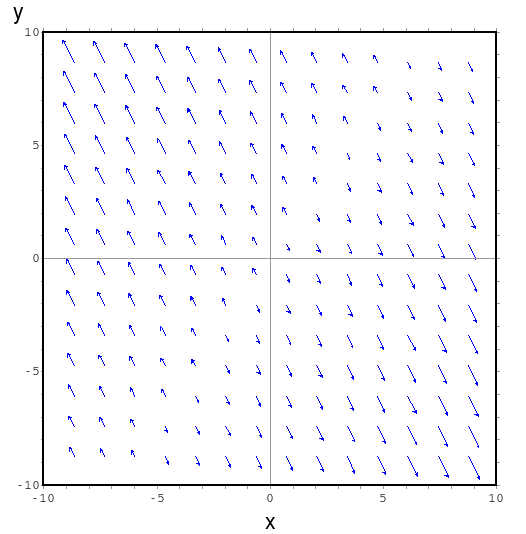
\includegraphics[width=0.5\textwidth]{de5}\end{center}	
\end{figure}\\}
Так как корни характеристического уравнения это действительные положительные числа, то точка покоя неустойчива и называется неустойчивым узлом(рисунок).\\
\\
\\
\\
\item[6.] Реализация метода сеток для дифференциальных уравнений в частных производных.\\
Пример 1. \\
\( \left\{
\begin{array}{l}
u_{xx}=\dfrac{1}{a^{2}}u_{tt}, \ 0\leq x\leq m, \ 0\leq y\leq n \\
u(x,0)=\sin(\pi x/50)\cos(\pi x), \ u_{t}(x,0)=0 \\
u(0,t)=u(m,t)=0.
\end{array} \right. \) \\
Вводим сетку: m=100 , n=200 , h=1 . Создаем нулевой массив значений \(U(i,j)\) размера m x n.\\
\texttt{\$m:42\$n:30\$ h:1\$;}

\texttt{for i:1 thru m do for j:1 thru n do}

\texttt{(arraymake (u,[i,j]), u[i,j]:0)\$;}\\
Задаем значения a=1, k=0,01.\\
\texttt{a:1\$k:0.01\$;}\\
Заполняем первую и вторую строки массива U начальными условиями \(u(x,0)=\sin(\pi x/9)\cos(\pi x), \ u_{t}(x,0)=0\) (нулевой начальной скорости соответствует совпадение значений (смещений) в первом и втором столбцах).\\
\texttt{for j:1 thru n do}\\
\texttt{(u[1,j]:sin(\%pi*j/9)*cos(\%pi*j), u[2,j]:u[1,j])\$;}\\
Заполняем первый и последний столбец массива U граничными условиями \(u(0,t)=u(m,t)=0\) (на концах струны смещение равно нулю в любой момент времени).\\
\texttt{for i:1 thru m do (u[i,1]:0, u[i,n]:0)\$;}\\
Находим решение, используя разностную схему\\
\(u_{i+1,j}=\dfrac{a^2 k^2}{h^2}[u_{i,j+1}-2u_{i,j}+u_{i,j-1}]+2u_{i,j}-u_{i-1,j}.\)\\
\texttt{for i:2 thru m-1 do for j:2 thru n-1 do}\\
\texttt{u[i+1,j]:float((a*k/h)\^{}2*(u[i,j+1]-}\\
\texttt{2*u[i,j]+u[i,j-1])+2*u[i,j]-u[i-1,j]),numer\$;}\\
Для вывода полученного решения в виде поверхности преобразуем наш массив U в функцию двух переменных:\\
\texttt{f(x,y):=float(u[round(x),round(y)])\$;}\\
Теперь выполняем построение:\\
\texttt{plot3d(f, [x,1,m], [y,1,n], [plot\_format, gnuplot])\$;}
\begin{figure}[h]
%\includegraphics[width=0.7\textwidth]{setka}
\end{figure}\\
\end{itemize}

\section*{ЗАКЛЮЧЕНИЕ}
\addcontentsline{toc}{section}{ЗАКЛЮЧЕНИЕ}
will be added 


\section*{СПИСОК ИСПОЛЬЗОВАННЫХ ИСТОЧНИКОВ}
\addcontentsline{toc}{section}{СПИСОК ИСПОЛЬЗОВАННЫХ ИСТОЧНИКОВ}
\begin{itemize}
\item[1] Ильин В. А., Позняк Э. Г. Линейная алгебра. М. : Наука, 1984. 294с.
\item[2] Берсенев С. М., Иванов И. О. О вычислительных схемах метода регуляризации  // Журн. вычисл. мат. и мат. физ. 1984. Т. 24, № 9. 1402–1405c. 
\item[3] Фомин А. Е. О компонентах групп // Исследования по теории групп: сб. науч. тр. Свердловск, 1984. 136–148c.
\item[4] Хромов А. П. Конечномерные возмущения вольтерровых операторов: дис. ... д-ра физ.-мат. наук. Новосибирск, 1973. 242с.
\item[5] Губина Т. Н., Андропова Е.В. Решение дифференциальных уравнений в системе компьютерной математике Maxima: Учебное пособие. Елец. 2009. 99с.
\item[6] Стахин Н. А. Основы работы с системой аналитических вычислений Maxima: Учебное пособие. М. 2008. 86с.
\item[7] Виноградов И. М. Математическая энциклопедия. М.: Советская энциклопедия. 1977—1985.
\end{itemize}
\end{document}